\documentclass{ximera}
\input{../preamble.tex}
\author{}
\license{Creative Commons 4.0 By-NC-SA}
%\outcome{Compute an antiderivative using basic formulas}
\begin{document}
\begin{exercise}

Determine whether each set, $S$, of vectors is closed under vector addition, and scalar multiplication. 

Let $S$ be the set of all vectors contained in a sphere of radius 1 centered at the origin.

\begin{center}
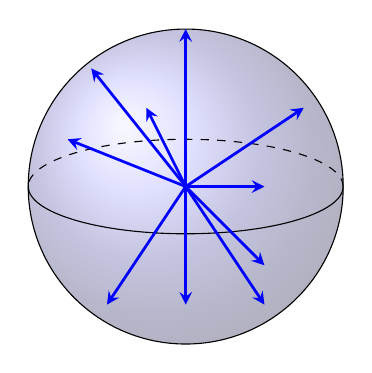
\begin{tikzpicture}
  \shade[ball color = blue!40, opacity = 0.4] (0,0) circle (2cm);
  \draw (0,0) circle (2cm);
  \draw (-2,0) arc (180:360:2 and 0.6);
  \draw[dashed] (2,0) arc (0:180:2 and 0.6);
  \fill[fill=black] (0,0) circle (1pt);

  \draw[->,line width=1pt,blue,-stealth](0,0)--(-1.2,1.5);
\draw[->,line width=1pt,blue,-stealth](0,0)--(1,0);
\draw[->,line width=1pt,blue,-stealth](0,0)--(0,-1.5);
\draw[->,line width=1pt,blue,-stealth](0,0)--(1,-1);
\draw[->,line width=1pt,blue,-stealth](0,0)--(-1,-1.5);
\draw[->,line width=1pt,blue,-stealth](0,0)--(1.5,1);
\draw[->,line width=1pt,blue,-stealth](0,0)--(0,2);
\draw[->,line width=1pt,blue,-stealth](0,0)--(-1.5,0.6);
\draw[->,line width=1pt,blue,-stealth](0,0)--(1,-1.5);
\draw[->,line width=1pt,blue,-stealth](0,0)--(-0.5,1);
\end{tikzpicture}
\end{center}

\begin{selectAll}
 \choice{$S$ is closed under scalar multiplication.}
 \choice{$S$ is closed under vector addition.}
 \choice[correct]{None of the above.}
 \end{selectAll}

Let $S$ be the set of all vectors contained in an infinite double cone.
\begin{center}
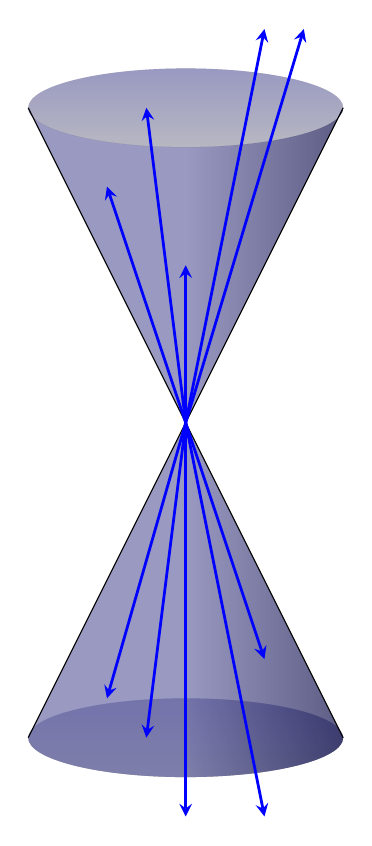
\begin{tikzpicture}
\fill[
  top color=blue!40,
  bottom color=blue!10,
  shading=axis,
  opacity=0.4
  ] 
 (0,4) circle (2cm and 0.5cm);

 \fill[
  top color=blue!40,
  bottom color=blue!10,
  shading=axis,
  opacity=0.4
  ] 
 (0,-4) circle (2cm and 0.5cm);
 
\fill[
  left color=blue!40!white,
  right color=blue!40!black,
  middle color=blue!40,
  shading=axis,
  opacity=0.4
  ] 
  (2,-4) -- (0,0) -- (-2,-4) arc (180:360:2cm and 0.5cm);

\fill[
  left color=blue!40!white,
  right color=blue!40!black,
  middle color=blue!40,
  shading=axis,
  opacity=0.4
  ] 
  (2,4) -- (0,0) -- (-2,4) arc (180:360:2cm and 0.5cm);
  
\draw 
  (-2,-4) -- (2,4);  

  \draw 
  (2,-4) -- (-2,4);  

\draw[->,line width=1pt,blue,-stealth](0,0)--(-1,3);
\draw[->,line width=1pt,blue,-stealth](0,0)--(1,5);
\draw[->,line width=1pt,blue,-stealth](0,0)--(0,-5);
\draw[->,line width=1pt,blue,-stealth](0,0)--(1,-3);
\draw[->,line width=1pt,blue,-stealth](0,0)--(-1,-3.5);
\draw[->,line width=1pt,blue,-stealth](0,0)--(1.5,5);
\draw[->,line width=1pt,blue,-stealth](0,0)--(0,2);
\draw[->,line width=1pt,blue,-stealth](0,0)--(-0.5,4);
\draw[->,line width=1pt,blue,-stealth](0,0)--(1,-5);
\draw[->,line width=1pt,blue,-stealth](0,0)--(-0.5,-4);
\end{tikzpicture}
\end{center}

\begin{selectAll}
 \choice[correct]{$S$ is closed under scalar multiplication.}
 \choice{$S$ is closed under vector addition.}
 \choice{None of the above.}
 \end{selectAll}
\end{exercise}
\end{document}